\documentclass[conference]{IEEEtran}
\IEEEoverridecommandlockouts
\usepackage{cite}
\usepackage{amsmath,amssymb,amsfonts}
\usepackage{graphicx}
\usepackage{booktabs}
\usepackage{xcolor}
\usepackage{url}
\usepackage[hidelinks]{hyperref}

\graphicspath{{conf_fig/}}

\begin{document}

\title{Explainable Cyberbullying Detection Using Deep Learning and Transformer Models with LIME}

\author{
\IEEEauthorblockN{Mohammad Asmual Hoque Yousha}
\IEEEauthorblockA{\textit{Dept.\ of Computer Science and Engineering} \\
\textit{Premier University}\\
Chattogram, Bangladesh \\
mdyousha138@gmail.com}
\and
\IEEEauthorblockN{Md Mostafa Kamal Anna}
\IEEEauthorblockA{\textit{Dept.\ of Computer Science and Engineering} \\
\textit{Premier University}\\
Chattogram, Bangladesh \\
mostafakamalanna88@gmail.com}
}

\maketitle

\begin{abstract}
Cyberbullying on social media is a growing problem, and the volume of user-generated text makes manual moderation impractical. Automatic detection has become an active research area, yet most detectors report only an aggregate score and give no reason for a decision, which limits how far they can be trusted. This paper presents a detector that is both accurate and explainable. We assemble a binary dataset of roughly 4{,}000 English comments, combining about 1{,}000 collected from YouTube, Reddit, and Facebook with about 3{,}000 derived from the Jigsaw toxic-comment corpus, and compare four models under identical conditions: a TF--IDF Logistic Regression baseline, an LSTM, a GRU, and a fine-tuned RoBERTa. RoBERTa performs best, reaching 92.33\% accuracy and F1, against 87.33\% for LSTM, 85.33\% for GRU, and 83.33\% for Logistic Regression. Running the same pipeline on the base paper's own 46{,}017-comment Twitter data, RoBERTa reaches 89.01\%, well above the base paper's reported 77.00\%, and it remains the best model in a four-way comparison against a second study. The central contribution is the addition of Local Interpretable Model-agnostic Explanations (LIME), which explains every prediction at the level of contributing words; neither comparison study offers this. The LIME analysis confirms that correct decisions rest on sensible words and also exposes a genuine weakness on sarcasm.
\end{abstract}

\begin{IEEEkeywords}
cyberbullying detection, RoBERTa, LIME, explainable AI, text classification, deep learning
\end{IEEEkeywords}

\section{Introduction}
Online communication has become one of the main ways people talk to each other, and the same platforms that make this possible also make it easy to hurt others at scale. A share of the comments posted every day on YouTube, Reddit, and Facebook is hostile, threatening, or demeaning, and for younger users in particular the effect of this kind of abuse on mental health is well documented~\cite{review2023dl}. Manual moderation cannot keep pace with the volume, which has made automatic cyberbullying detection an active research problem.

Machine learning and, more recently, transformer-based language models have pushed accuracy upward on this task. A practical concern, however, remains largely unaddressed: most published detectors report only a label and a probability and give no insight into \emph{why} a comment was flagged. For a system that may lead to a post being removed or a user being warned, this opacity is a real limitation, because a moderator or an affected user has good reason to ask which words drove the decision. The base paper we extend, Esan \emph{et al.}~\cite{esan2024lstm}, is a clear example: it reports an LSTM at 77.00\% accuracy with no interpretability of any kind.

This paper addresses both accuracy and transparency together. We frame cyberbullying detection as binary classification, compare four models spanning the classical-to-transformer range, and pair the best model with LIME~\cite{ribeiro2016lime} so that every prediction can be traced back to the words that mattered. Our contributions are: (i) a fine-tuned RoBERTa detector that reaches 92.33\% accuracy on our combined data, well above the base paper; (ii) cross-dataset validation showing the improvement holds on the base paper's own data; and (iii) a LIME-based explainability layer that neither of our two comparison studies provides, which not only builds trust but also, as we show, exposes a concrete failure mode on sarcasm.

\section{Related Work}
Detection of abusive online content is usually cast as supervised classification over short texts. Early work relied on hand-built features fed to classical classifiers; the field then moved through recurrent networks such as LSTM~\cite{hochreiter1997lstm} and GRU~\cite{cho2014gru}, and on to pretrained transformers. The transformer architecture~\cite{vaswani2017attention} and BERT~\cite{devlin2019bert} set new records across NLP, and RoBERTa~\cite{liu2019roberta} refined BERT's pretraining and improved on it. Because these models arrive already knowing a great deal about language, fine-tuning them on a modest dataset tends to beat recurrent models trained from scratch.

Within cyberbullying specifically, Esan \emph{et al.}~\cite{esan2024lstm} report an LSTM at 77.00\% on a Kaggle Twitter dataset with no explanations, and Ogunleye and Dharmaraj~\cite{ogunleye2023llm} report RoBERTa at about 87\% on an English FormSpring/Twitter set, again without interpretability. Other studies push accuracy higher through heavier pipelines, such as the stacking ensemble of Muneer \emph{et al.}~\cite{muneer2023stacking} and the GloVe-augmented RoBERTa of Alrowais~\cite{alrowais2024robertanet}, but none explains individual decisions. Explainability is the gap we target: LIME~\cite{ribeiro2016lime} is model-agnostic, local, and word-level, which suits a moderator reviewing a single flagged comment.

\section{Methodology}
Fig.~\ref{fig:pipeline} summarises the pipeline, which is applied identically to every model so that comparisons are fair.

\begin{figure}[t]
\centering
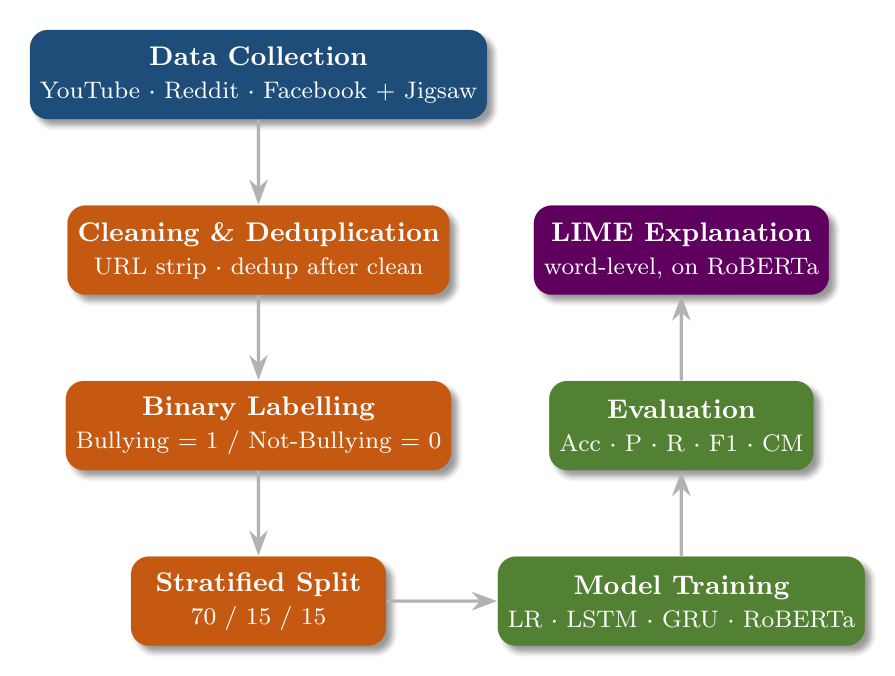
\includegraphics[width=\columnwidth]{diag_pipeline.png}
\caption{End-to-end pipeline: data collection, cleaning and deduplication, binary labelling, stratified splitting, model training, evaluation, and LIME explanation on the best model.}
\label{fig:pipeline}
\end{figure}

\subsection{Dataset}
We combine two sources into roughly 4{,}000 English comments. About 1{,}000 were collected by hand from YouTube, Reddit, and Facebook and quality-filtered; about 3{,}000 were derived from the Jigsaw Toxic Comment corpus~\cite{jigsaw}. Collecting from several platforms exposes the models to a wider range of writing styles than any single source would. Every comment is reduced to a single binary label, and the classes are close to balanced (2{,}059 Not-Bullying, 1{,}941 Bullying), so accuracy is a meaningful summary.

\subsection{Preprocessing}
Cleaning is deliberately light: URLs are stripped and whitespace is normalised. One ordering choice matters, namely that deduplication is performed \emph{after} cleaning; near-duplicates that differ only by a trailing URL or spacing survive a naive pass but collapse once cleaning removes those surface differences, and catching them prevents leakage across the train/test boundary.

\subsection{Models}
Four models are trained: a TF--IDF Logistic Regression ($C=1$, unigrams and bigrams, 10k features); an LSTM and a GRU (128-dim embedding, two recurrent layers of 128 and 64 units, dropout 0.3, sequence length 100); and a fine-tuned \texttt{roberta-base} (max length 128, AdamW at $2\times10^{-5}$, batch 32, up to 6 epochs with early stopping on validation loss). The data is shuffled with a fixed seed and split $70/15/15$ with stratification, and the same split is reused for all models.

\subsection{Explainability}
LIME explains one prediction at a time by perturbing the comment (removing subsets of words), recording how RoBERTa's predicted probability changes, and fitting a simple weighted linear model locally; its coefficients give each word a signed importance. Each explanation uses 10 features and 500 perturbation samples. The output for a comment is its predicted class, a confidence, and a ranked list of words with signed weights.

\subsection{Evaluation}
All models are scored on the held-out test set using accuracy, precision, recall, and F1 (weighted), with confusion matrices for inspection.

\section{Results and Discussion}
\subsection{Model Performance}
Table~\ref{tab:results} reports the four models on the 600-comment test set. The ordering is the one the literature predicts: the linear baseline is solid, the recurrent models improve on it, and RoBERTa is clearly ahead, five points above the best recurrent model, with its four metrics tracking each other closely.

\begin{table}[t]
\caption{Performance of the Four Models (Test Set, $n=600$)}
\label{tab:results}
\centering
\begin{tabular}{lcccc}
\toprule
\textbf{Model} & \textbf{Acc.} & \textbf{Prec.} & \textbf{Rec.} & \textbf{F1} \\
\midrule
Logistic Regression & 83.33 & 83.62 & 83.33 & 83.27 \\
GRU & 85.33 & 85.36 & 85.33 & 85.34 \\
LSTM & 87.33 & 87.33 & 87.33 & 87.33 \\
\textbf{RoBERTa (ours)} & \textbf{92.33} & \textbf{92.36} & \textbf{92.33} & \textbf{92.33} \\
\bottomrule
\end{tabular}
\end{table}

\subsection{Confusion Matrices}
Fig.~\ref{fig:cm} places all four confusion matrices on one scale. Every model keeps a dark diagonal, but Logistic Regression has lopsided errors (65 missed bullying comments against 35 false positives), the recurrent models cut the misses by modelling word order, and RoBERTa has the fewest and best-balanced errors, 19 false positives and 27 misses.

\begin{figure*}[t]
\centering
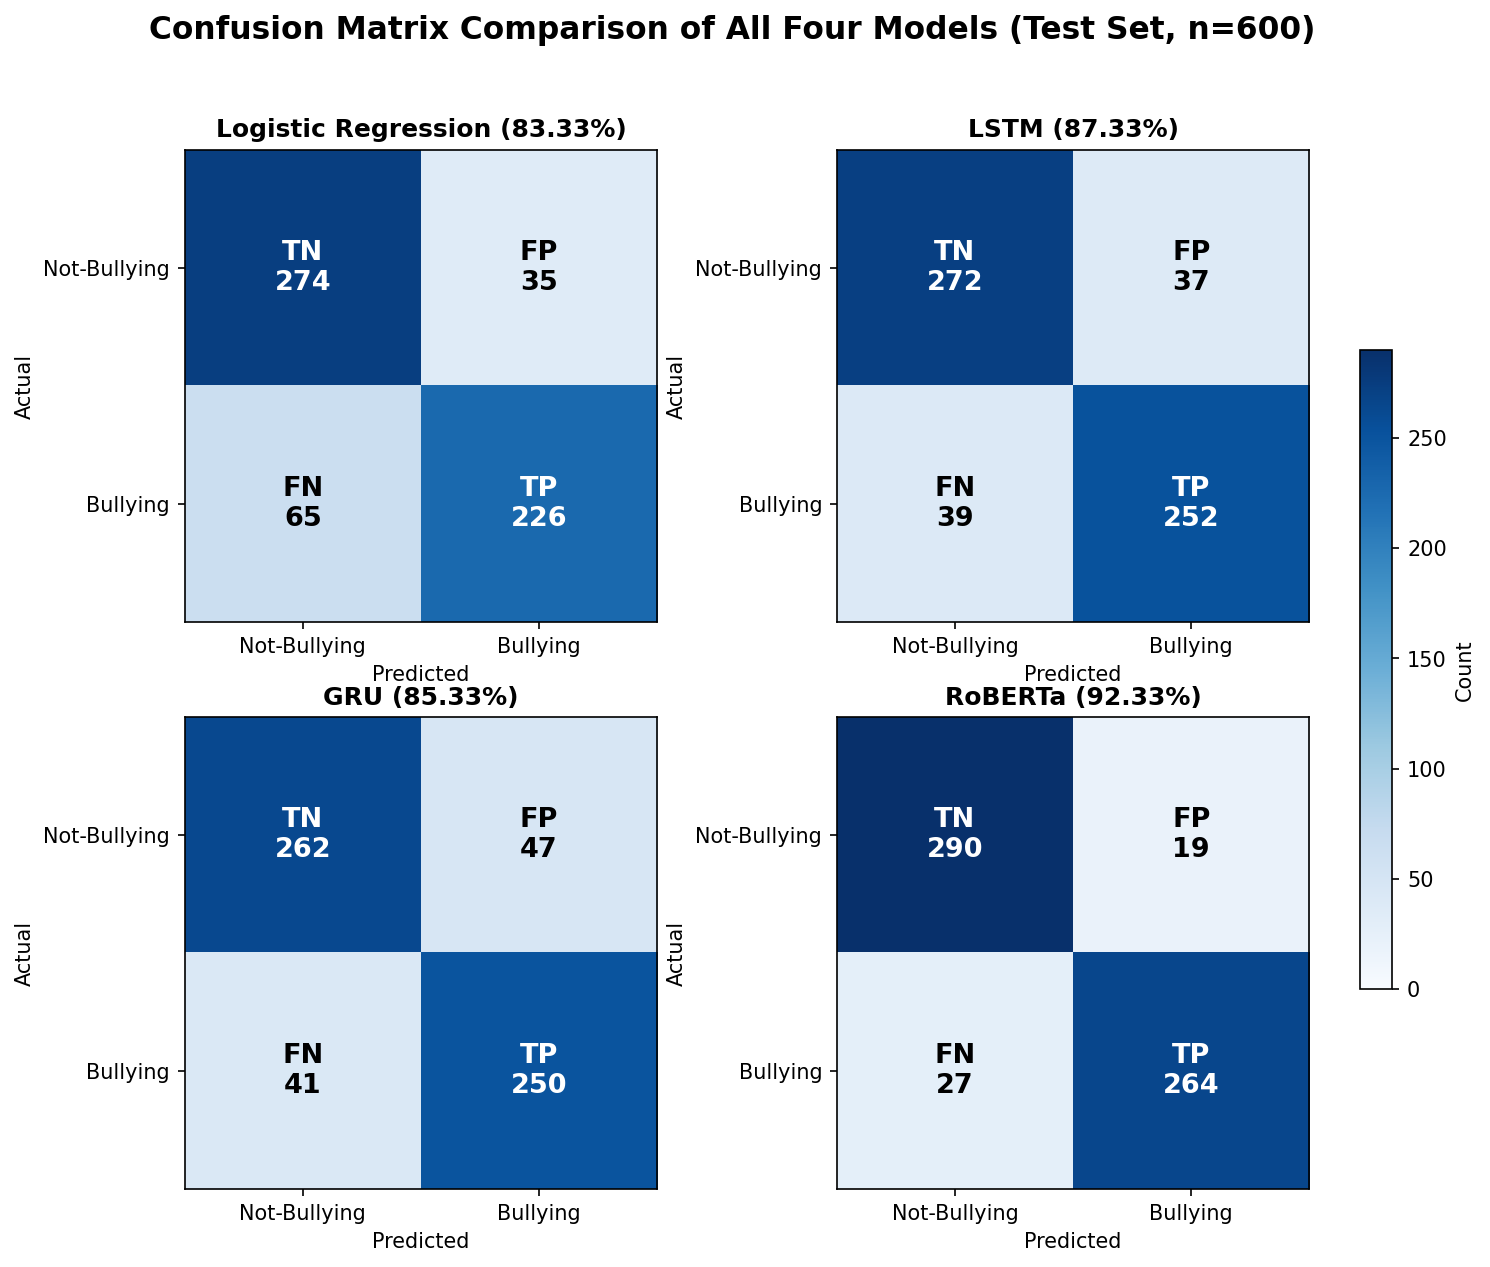
\includegraphics[width=0.78\textwidth]{cm_combined.png}
\caption{Confusion matrices of all four models on the test set ($n=600$) on a shared colour scale. RoBERTa (bottom-right) has the fewest and most balanced errors.}
\label{fig:cm}
\end{figure*}

\subsection{Comparison with Prior Work}
Comparing headline numbers across different data would be unfair, so we ran our pipeline on the base paper's own 46{,}017-comment Twitter data. There our RoBERTa reaches 89.01\% and even the recurrent and linear models land in the high 86\% range, all far above the base paper's 77.00\%~\cite{esan2024lstm}. Against the second study~\cite{ogunleye2023llm}, whose code and data are public, we ran a four-way comparison (our data/their data $\times$ our code/their code); RoBERTa was the best model in every setting, reaching 92.33\% on our data and 89.79\% on their data, both above their published 87.00\%. One result we report plainly: their implementation reached 95.25\% on our own data, higher than our 92.33\% on the same data, which isolates training and implementation details as a factor worth pursuing in future work.

\subsection{Explainability}
Accuracy says how often a model is right but nothing about why. Applied to RoBERTa, LIME makes the reasoning visible. For ``Everyone hates you, just go away'' (Bullying, 93.30\%) the decision rests on \emph{hates}, \emph{you}, and \emph{away}, exactly what a human would point to. The most instructive case is a failure: ``Wow, you're really smart... said no one ever.'' is sarcastic mockery but was labelled Not-Bullying with 95.32\% confidence. Fig.~\ref{fig:lime} shows why, as the surface-positive words \emph{Wow}, \emph{really}, and \emph{said} pull toward Not-Bullying and the reversal carried by ``said no one ever'' is never captured. This error would be invisible from the aggregate metrics; it only becomes legible once the prediction is explained, which is the whole argument for building explainability into the system.

\begin{figure}[t]
\centering
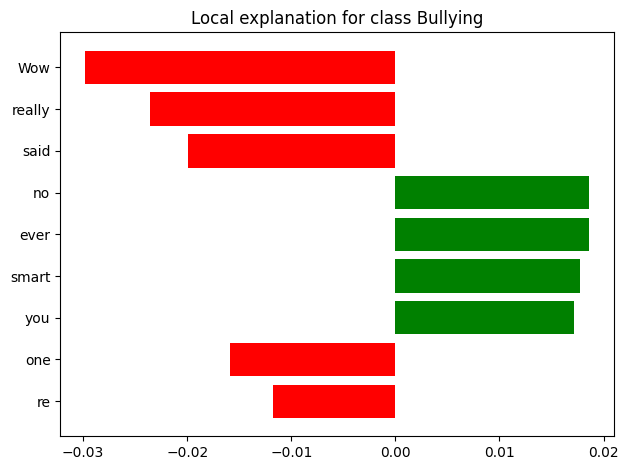
\includegraphics[width=0.95\columnwidth]{lime_sarcasm.png}
\caption{LIME for the misclassified sarcastic comment. Positive-sounding words (red) drive the wrong Not-Bullying prediction.}
\label{fig:lime}
\end{figure}

\subsection{Error Analysis}
Beyond sarcasm, errors cluster around very short comments, where there is little evidence to weigh, and around strongly worded but non-targeting comments, where the model occasionally reads intensity as hostility. These patterns are consistent with RoBERTa's roughly balanced false positives and false negatives.

\section{Conclusion and Future Work}
We presented a cyberbullying detector that is both accurate and explainable. A fine-tuned RoBERTa reached 92.33\% on our combined multi-platform data and stayed the best model on the base paper's data and in a four-way comparison, while LIME turned each decision into an inspectable, word-level explanation that neither comparison study offers. The broader point is that accuracy and transparency need not be traded against each other. Future work follows directly from the limitations we found: closing the training gap behind the external implementation, making the model sarcasm-aware, restoring the fine-grained bullying types we recorded but did not use, and extending the detector to Bangla and English (and, where data allows, Hindi) for multilingual and code-mixed text.

\begin{thebibliography}{00}
\bibitem{esan2024lstm} O.~Abodunrin \emph{et al.}, ``LSTM-based model for cyberbully detection,'' \emph{LAUTECH J. Eng. Technol.}, vol.~18, no.~1, pp.~181--191, 2024.
\bibitem{ogunleye2023llm} B.~Ogunleye and B.~Dharmaraj, ``The use of a large language model for cyberbullying detection,'' \emph{Analytics}, vol.~2, no.~3, pp.~694--707, 2023.
\bibitem{ribeiro2016lime} M.~T.~Ribeiro, S.~Singh, and C.~Guestrin, ```Why should I trust you?': Explaining the predictions of any classifier,'' in \emph{Proc. 22nd ACM SIGKDD}, 2016, pp.~1135--1144.
\bibitem{liu2019roberta} Y.~Liu \emph{et al.}, ``RoBERTa: A robustly optimized BERT pretraining approach,'' \emph{arXiv:1907.11692}, 2019.
\bibitem{devlin2019bert} J.~Devlin, M.-W.~Chang, K.~Lee, and K.~Toutanova, ``BERT: Pre-training of deep bidirectional transformers for language understanding,'' in \emph{Proc. NAACL-HLT}, 2019, pp.~4171--4186.
\bibitem{vaswani2017attention} A.~Vaswani \emph{et al.}, ``Attention is all you need,'' in \emph{Proc. NeurIPS}, vol.~30, 2017.
\bibitem{hochreiter1997lstm} S.~Hochreiter and J.~Schmidhuber, ``Long short-term memory,'' \emph{Neural Comput.}, vol.~9, no.~8, pp.~1735--1780, 1997.
\bibitem{cho2014gru} K.~Cho \emph{et al.}, ``Learning phrase representations using RNN encoder--decoder for statistical machine translation,'' in \emph{Proc. EMNLP}, 2014, pp.~1724--1734.
\bibitem{muneer2023stacking} A.~Muneer \emph{et al.}, ``Cyberbullying detection on social media using stacking ensemble learning and enhanced BERT,'' \emph{Information}, vol.~14, no.~8, art.~467, 2023.
\bibitem{alrowais2024robertanet} F.~Alrowais, ``RoBERTaNET: Enhanced RoBERTa transformer based model for cyberbullying detection with GloVe features,'' \emph{IEEE Access}, vol.~12, 2024.
\bibitem{review2023dl} M.~T.~Hasan \emph{et al.}, ``A review on deep-learning-based cyberbullying detection,'' \emph{Future Internet}, vol.~15, no.~5, art.~179, 2023.
\bibitem{jigsaw} Jigsaw and Conversation AI, ``Toxic comment classification challenge,'' Kaggle, 2018.
\end{thebibliography}

\end{document}
